\documentclass{standalone}

\usepackage[usenames,dvipsnames]{xcolor}
\usepackage{tikz}
\usetikzlibrary{shapes,shadows,calc}
\usepackage{subfigure}




\begin{document}

 \begin{center}
  
  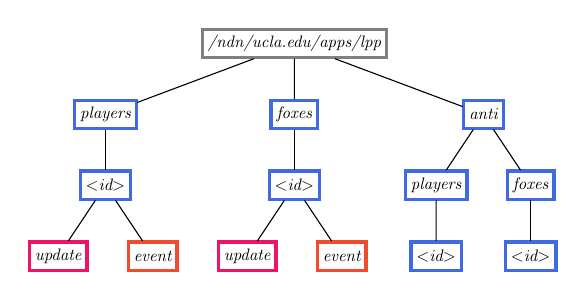
\begin{tikzpicture} [scale=0.6, transform shape,
				state/.style={
				% The shape:
				rectangle,
				% The size:
      				minimum size=6mm,
				% The border:
      				 very thick,
     				 draw=WildStrawberry,
      				% The filling:
				%fill=Rhodamine,
				%top color=white,
				%bottom color=white, % and something else at the bottom % Font
				font=\itshape
    				},
				asset/.style={
				% The shape:
				rectangle,
				% The size:
      				minimum size=6mm,
				% The border:
      				very thick,draw=RoyalBlue,
      				% The filling:
				%top color=white,
				%bottom color=cyan!50!black!20!, % and something else at the bottom % Font
				font=\itshape
    				},
				event/.style={
				% The shape:
				rectangle,
				% The size:
      				minimum size=6mm,
				% The border:
      				very thick,draw=RedOrange,
      				% The filling:
				%top color=white,
				%bottom color=Dandelion, % and something else at the bottom % Font
				font=\itshape
    				},
				default/.style={
				% The shape:
				rectangle,
				% The size:
      				minimum size=6mm,
				% The border:
      				very thick,draw=Gray,
   				%top color=white,
				%bottom color=Gray,
      				% The filling:
				font=\itshape
    				},
				]
    \tikzstyle{every node} = [align=center]
   % \tikzstyle{asset} = [fill=cyan!15]
   % \tikzstyle{state} = [fill=magenta!15]
   % \tikzstyle{event} = [fill=orange!15]
    \tikzstyle{level 1} = [sibling distance=40mm]
    \tikzstyle{level 2} = [sibling distance=20mm]
    \node [default] {/ndn/ucla.edu/apps/lpp}
        child { node [asset] {players} 
		child { node [asset] {$<$id$>$} 
			child { node [state] {update}}
			child { node [event] {event}}
		}
        }
        child{ node[asset] {foxes}
        		child{ node [asset] {$<$id$>$}
			child { node [state] {update}}
			child { node [event] {event}}
		}
        }
         child{ node [asset] {anti}
        		child { node [asset] {players}
			child { node [asset] {$<$id$>$}}
		}
		child { node [asset] {foxes}
			child { node [asset] {$<$id$>$}}
		}
        }
    ;
\end{tikzpicture}


\end{center}


\end{document}